\documentclass[conference]{IEEEtran}
\IEEEoverridecommandlockouts

\usepackage{amsmath}
\usepackage{amssymb}
\usepackage{graphicx}
\usepackage{booktabs}
\usepackage{multirow}
\usepackage{url}
\usepackage{hyperref}
\usepackage{xcolor}

\def\BibTeX{{\rm B\kern-.05em{\sc i\kern-.025em b}\kern-.08em T\kern-.1667em\lower.7ex\hbox{E}\kern-.125emX}}

\begin{document}

\title{A Validated LLM-as-Judge Framework for Detecting Evasion in Institutional Question-Answering, with an Application to Earnings Calls}

\author{
\IEEEauthorblockN{Kunal Chevuri}
\IEEEauthorblockA{University of North Texas\\Denton, TX\\kunalchevuri510@gmail.com}
\and
\IEEEauthorblockN{Ayaan Sheikh}
\IEEEauthorblockA{University of North Texas\\Denton, TX\\ayaansarfrazsheikh@gmail.com}
\and
\IEEEauthorblockN{Mohammed Aledhari}
\IEEEauthorblockA{University of North Texas\\Denton, TX\\Mohammed.Aledhari@unt.edu}
}

\maketitle

\begin{abstract}
Institutional settings frequently place decision-makers in live, unscripted question-and-answer exchanges---congressional hearings, regulatory proceedings, central bank press conferences, and corporate earnings calls---where responses may substantively engage with what was asked or evade it. We introduce a structured LLM-as-judge framework that scores evasiveness along four interpretable dimensions---non-responsiveness, vagueness, deflection, and hedging---and apply it at scale to 3,350 question-response pairs drawn from 285 SEC-filed earnings call transcripts spanning 49 companies and the years 2015 to 2023. We validate the automated scoring against independent human annotation on a stratified sample of 75 pairs, finding modest agreement on discrete evasion categories but strong agreement on the underlying continuous scale (Pearson $r = 0.59$ to $0.80$ across rater comparisons), indicating the framework captures real, human-interpretable variation in response quality rather than model idiosyncrasy. As an illustrative application, we test whether transcript-level evasion predicts subsequent market reactions to earnings announcements, motivated by voluntary disclosure theory. In a final sample of 155 firm-quarter observations, we find no significant relationship, a result that holds under cross-validation, COVID-period exclusion, and a formal power analysis, and we report this honestly as a boundary condition on the framework's financial applicability rather than obscuring it. We position the paper's central contribution as the validated measurement framework itself: a fully reproducible, publicly-sourced pipeline for detecting evasion in adversarial institutional Q\&A, directly extensible to settings well beyond corporate disclosure.
\end{abstract}

\begin{IEEEkeywords}
large language models, LLM-as-judge, institutional question-answering, earnings calls, textual analysis, financial technology, automated model evaluation, natural language processing
\end{IEEEkeywords}

\section{Introduction}

Many important institutional settings share a common structure: a decision-maker faces live, unscripted questioning from an interlocutor with the standing to demand a real answer---an analyst on an earnings call, a journalist at a press conference, a legislator in a hearing---and the responses given, or not given, carry information. Distinguishing a substantive answer from an evasive one is intuitive to a human listener but has proven difficult to measure systematically at scale. This paper introduces a tool for exactly that task: a structured large language model (LLM) judge that scores the evasiveness of a response along four interpretable dimensions---non-responsiveness, vagueness, deflection, and hedging---validated against independent human judgment and built entirely from public data and open methodology.

We develop and validate this framework using corporate earnings calls as our testbed, given the availability of full, unscripted question-and-answer transcripts filed publicly with the U.S. Securities and Exchange Commission (SEC). We apply our LLM judge (\texttt{claude-sonnet-4-6}, temperature 0) to 3,350 question-response pairs drawn from 285 transcripts across 49 companies and the 2015--2023 period, and validate its output against independent human annotation on a stratified sample of 75 pairs. While human raters do not always agree with each other or the model on precise categorical labels---a genuinely subjective task---agreement on the underlying continuous evasion scale is strong, indicating the framework captures real signal.

As an illustrative application, we then test the following hypothesis: \textbf{H1}: transcript-level evasion is negatively associated with the market reaction to the subsequent earnings announcement, following voluntary disclosure theory's prediction that evasive responses may signal undisclosed unfavorable information. We report this honestly: in a final sample of 155 firm-quarter observations, evasion does not significantly predict subsequent abnormal returns, a null result we stress-test extensively via cross-validation and a formal power analysis rather than allowing a single favorable specification to stand unexamined.

We regard this paper's contribution as the measurement framework itself, not the specific financial application: the framework is directly extensible to any adversarial institutional question-and-answer setting, and we view the earnings call test as a rigorous illustration of how the tool should be applied and evaluated---including reporting when a downstream hypothesis is not supported---rather than as a verdict on the framework's broader usefulness. A reader should weigh the framework's demonstrated reliability independently of whether this particular financial hypothesis is supported.

\section{Related Literature}

This paper draws on four literatures: LLM-as-judge methodology, earnings call linguistics, equivocation theory, and voluntary disclosure theory.

\textbf{LLM-as-judge methodology.} Large language models have recently been established as viable substitutes for human evaluators in subjective text-scoring tasks. Zheng et al.~\cite{zheng2023judging} show instruction-tuned LLMs can approximate human preference judgments with high agreement, introducing the ``LLM-as-judge'' paradigm now widely used to benchmark generative systems; Dubois et al.~\cite{dubois2024length} extend this with length-controlled evaluation protocols addressing known biases in automated judging, and Liu et al.~\cite{liu2023geval} introduce G-Eval, a chain-of-thought-based LLM evaluation framework closely related to our structured rubric approach. This literature, and the associated judge-bias concerns it has identified (position, verbosity, and self-preference biases), has been applied almost exclusively to benchmarking model outputs against one another; extending it to detect strategic communicative behavior in real institutional settings is this paper's core methodological contribution.

\textbf{Earnings call linguistics and closely related recent work.} Larcker and Zakolyukina~\cite{larcker2012detecting} link deceptive or evasive linguistic patterns in earnings call narratives to subsequent financial misstatements, while Jiang et al.~\cite{jiang2019manager} and Keith and Stent~\cite{keith2019modeling} apply sentiment and semantic analysis to prepared remarks and analyst question framing, respectively. Two recent efforts are closely related to our approach and warrant direct engagement. Ma et al.~\cite{ma2026evasionbench} introduce EvasionBench, a large-scale benchmark for managerial evasion in earnings-call Q\&A: 22.7 million raw pairs extracted from S\&P Capital IQ transcripts, filtered down to an 84,000-pair training set and a 1,000-pair human-labeled gold test set, built on a three-level taxonomy with multi-model-consensus annotation, achieving substantially higher human agreement (their reported $\kappa = 0.835$) than we observe here; their fine-tuned Eva-4B model attains 84.9 percent Macro-F1 on that gold set. The gold split itself is not part of their public release---the distributed corpus carries labels generated by their Eva-4B-V2 model---which constrains how external evaluation against it can be interpreted, as we discuss in Section~\ref{sec:results}. Our approach differs in three ways: we use continuous, multi-dimensional, interpretable scoring rather than a single three-way label; we pair the measure with an explicit downstream market-reaction test; and we report a null result transparently rather than only the validation exercise. The higher agreement EvasionBench reports is a useful benchmark against which to read our own more modest categorical $\kappa$, and we view rubric design---particularly around explicit anchoring examples for each category---as a likely contributor to that gap. Separately, Thomas et al.~\cite{thomas2024never} introduce a two-level clarity and evasion taxonomy for political interview question-answering (the CLARITY/QEvasion line, since formalised as SemEval-2026 Task 6~\cite{thomas2026clarity}, in which 124 teams reached 0.89 Macro-F1 at the clarity level but only 0.68 on fine-grained evasion type), which is the natural language processing (NLP) lineage for our stated goal of generalizing beyond corporate disclosure to interviews and testimony; we evaluate against both corpora directly in Section~\ref{sec:results}. Two further 2025 contributions bracket our own. Al Nuaimi et al.~\cite{alnuaimi2025evasive} propose a psychological discourse taxonomy of seven evasion tactics for financial Q\&A together with lightweight baselines, sharing our interest in interpretable structure but stopping short of a downstream economic test. Bamber and Nappert~\cite{bamber2025nonanswers} approach the same phenomenon qualitatively, documenting that roughly 11 percent of analyst questions go unanswered and arguing that answers and non-answers are codependent rather than a simple signal of withheld bad news---a caution we take seriously in interpreting our own null.

\textbf{Reconciling a null with large-sample evidence.} Industry and benchmark-scale work reports that evasive disclosure carries measurable economic consequences, while our own downstream test (Section~\ref{sec:robustness}) does not. These are compatible, and it is worth stating why before the result is read as a contradiction. Three differences separate the settings. The samples differ by roughly two orders of magnitude: our analytical panel comprises 155 firm-quarters, against the tens of thousands of pairs available to corpus-scale studies. The measures differ: we regress a transcript-level mean of a continuous composite, whereas the comparison work typically classifies individual exchanges and aggregates differently. And the horizons differ: we test a three-day cumulative abnormal return around the subsequent announcement, a window chosen for identification rather than for power against slow-moving effects. Our post-hoc power analysis makes the implication concrete---at $n = 155$ the design has 34.4 percent power to detect an AUROC difference of 0.10 and 66.4 percent at 0.15. A null here therefore rules out a moderate-to-large effect in this sample; it is not evidence against the small effects that large samples are built to detect.

\textbf{Equivocation theory.} Our four rubric dimensions are, in substance, an operationalization of equivocation as studied in the communication literature~\cite{bull2003microanalysis,bull1993how,clayman2001answers,rasiah2010framework}, which analyzes how public figures respond to questions they would prefer not to answer directly. Grounding our rubric in this literature gives the measurement instrument a theoretical home beyond its immediate NLP and financial applications.

\textbf{Voluntary disclosure theory.} For our illustrative financial application, we draw on voluntary disclosure theory~\cite{dye1985disclosure,verrecchia2001essays}: managers with private information strategically withhold unfavorable disclosures when doing so is not fully unraveled by rational markets. This connects to a finance literature examining disclosure behavior around earnings communications directly. Hollander et al.~\cite{hollander2010silence} document that managers strategically decline to answer analyst questions during conference calls and that investors interpret such silence negatively. Most directly relevant, Gow et al.~\cite{gow2021nonanswers} construct a linguistic-analysis measure of ``non-answers'' during conference calls, finding roughly 11 percent of analyst questions receive non-answers and that performance-related and proprietary-information questions are especially likely to trigger them; our LLM-based approach can be read as an alternative, more flexible operationalization of the same underlying construct they measure with hand-crafted linguistic rules. Their 11 percent non-answer rate and our 2.84 percent high-evasion rate (pair-level score $\geq 60$) are not directly comparable, since the two measures use different underlying constructs and thresholds, but the gap is broadly consistent with our continuous score capturing a wider range of partial engagement than a binary non-answer label, with only the most extreme cases crossing our higher threshold. Barcellos~\cite{barcellos2025overcoming} examines how investor skepticism moderates the market's ability to detect deceptive evasion tactics in earnings calls (Articles in Advance at the time of writing; DOI: 10.1287/mnsc.2025.01197). Together these motivate our hypothesis that evasive responses may signal withheld unfavorable information, tested in Section~\ref{sec:results} and stress-tested further in Section~\ref{sec:robustness}.

\section{Methodology}
\label{sec:methodology}

We use a large language model as a structured judge to score evasion in question-response pairs. For each pair $(q_i, r_i)$ in transcript $t$, the judge produces four component scores on a five-point scale: non-responsiveness ($s_i^{NR}$), vagueness ($s_i^{V}$), deflection ($s_i^{D}$), and hedging ($s_i^{H}$). The pair-level evasion score rescales the mean of these components to $[0, 100]$:

\begin{equation}
E_i = \frac{\bar{s}_i - 1}{4} \times 100, \qquad \bar{s}_i = \frac{s_i^{NR} + s_i^{V} + s_i^{D} + s_i^{H}}{4}
\end{equation}

Transcript-level measures aggregate across all pairs in $t$: mean evasion $\bar{E}_t$, within-transcript variance $\sigma^2_{E,t}$, and maximum pair-level score $E_t^{max}$, the last capturing acute evasion on a single salient question even when overall tone is direct.

To validate the judge against human judgment, we built a parallel four-dimension rubric (topical alignment 0--3, specificity 0--3, completeness 0--2, deflection signals 0--2, inverted to a 0--10 evasion score), independently applied by two raters to 75 pairs. Because this human rubric is a related but not identical instrument to the LLM's own four dimensions, agreement between the two is best understood as a test of \emph{convergent validity}---whether two different measurement approaches targeting the same underlying construct converge---rather than agreement on an identical scale. We report unweighted and quadratic-weighted Cohen's $\kappa$ alongside Pearson correlation, since weighted $\kappa$ discounts near-miss adjacent-category disagreements that unweighted $\kappa$ penalizes fully. To further test whether the construct is model-independent, we additionally re-scored this sample with a second, architecturally distinct LLM.

As an illustrative downstream application of the validated framework, we test whether transcript-level evasion carries incremental predictive information about subsequent firm performance. We specify four nested feature configurations, where $y_t \in \{0, 1\}$ is the direction of the three-day cumulative abnormal return (CAR) around the firm's next earnings announcement and $CAR_t \in \mathbb{R}$ its magnitude:

\begin{align}
\text{A:}\ & \{\text{RevGrowth}, \text{GrossMargin}, \text{OpMargin}, \text{ROA}\}_t \\
\text{B:}\ & \text{A} \cup \{\text{LM}^+, \text{LM}^-, \text{LM}^{Unc}, \text{LM}^{Lit}\}_t \\
\text{C:}\ & \text{B} \cup \{\bar{E}_t\} \\
\text{D:}\ & \text{B} \cup \{\bar{E}_t, \sigma^2_{E,t}, E_t^{max}\}
\end{align}

Here RevGrowth, GrossMargin, and OpMargin are revenue growth, gross margin, and operating margin, and ROA is return on assets; LM$^+$, LM$^-$, LM$^{Unc}$, and LM$^{Lit}$ are the Loughran--McDonald~\cite{loughran2011liability} positive, negative, uncertainty, and litigious sentiment counts (defined fully in Section~\ref{sec:data}), named here to establish notation before that section's data description.

Each configuration is evaluated with logistic regression and XGBoost (max depth 3, 100 estimators), trained on a chronological 70 percent split and tested on the remaining 30 percent to respect temporal ordering. Missing accounting features are imputed using training-set medians; imputation is nontrivial for two features in particular (gross margin is observed for 109 of 155 observations, operating margin for 113 of 155), which we disclose explicitly given the scale of imputation involved. We compare Config C against B via the difference in test-set area under the receiver operating characteristic curve (AUROC) and a bootstrap 95 percent confidence interval (CI, 1,000 resamples), and additionally report 5-fold cross-validation and a post-hoc power analysis, treating this application as a test case for how the framework should be evaluated honestly rather than as the paper's central claim.

\section{Data and Experimental Design}
\label{sec:data}

Our corpus consists of earnings call transcripts filed as 8-K exhibits with the SEC, retrieved through the EDGAR Full-Text Search system using phrase-based filters designed to identify transcripts containing a live analyst Q\&A segment. Retrieval was necessarily lossy: of 22,596 8-K filings identified via the SEC submissions API for candidate companies over 2015--2023, 523 were confirmed via phrase-based search to contain a qualifying earnings-call transcript exhibit and successfully downloaded, with the large gap reflecting that most 8-K exhibits are not earnings-call transcripts at all, rather than retrieval failure in the conventional sense. This yielded 285 candidate transcripts spanning 49 unique companies and fiscal years 2015 through 2023, which we use purely as a large, realistic, and freely available testbed for the evasion-detection framework, not because earnings calls are the framework's intended sole application.

Each transcript was parsed to isolate the Q\&A section from preceding prepared remarks, using section-header detection adapted to multiple transcript formatting conventions. Speaker turns were classified as analyst questions or management responses using participant lists extracted from each transcript's header sections, with operator or moderator turns discarded. Consecutive analyst-management turn pairs were assembled into question-response units subject to minimum length filters (30 words per question, 50 words per response), yielding 3,350 scored pairs, each evaluated by the LLM judge described in Section~\ref{sec:methodology}. To assess reliability, a stratified sample of 75 pairs, spanning the corpus's full range of companies and years, was independently annotated by two human raters using the parallel rubric described above, without consulting one another or the model's output.

Table~\ref{tab:funnel} reports the retrieval funnel end to end, since the
attrition between filings identified and transcripts scored is large and is
easy to mistake for retrieval failure. It is not: the overwhelming majority of
8-K exhibits are not earnings-call transcripts at all. Raw filings are not
redistributed with our replication materials; they are re-fetchable from EDGAR
using the committed scraper, and the intermediate stage counts below are
reproducible from that point onward.

\begin{table}[t]
\centering
\caption{Retrieval and Processing Funnel}
\label{tab:funnel}
\begin{tabular}{lr}
\toprule
Stage & Count \\
\midrule
8-K filings identified, 2015--2023 & 22,596 \\
Confirmed transcript exhibits, downloaded & 523 \\
Transcripts clearing minimum-pair filters & 285 \\
Q\&A pairs extracted & 3,351 \\
Q\&A pairs scored & 3,350 \\
Unique companies & 49 \\
Firm-quarters in the analytical panel & 155 \\
\bottomrule
\end{tabular}
\end{table}

Scoring the full corpus is inexpensive, which matters for a method intended to
be reused. Across 3,350 pairs the judge consumed 2.67 million input and 0.32
million output tokens, costing \$12.77 at list price, or \$0.0038 per pair.
Token counts are measured with the provider's tokenizer over a 200-prompt
sample rather than approximated. Throughput, timed on the same call path, is
3.0 seconds per pair serially and 2.67 pairs per second at eight concurrent
workers, so the full corpus rescores in roughly 21 minutes. One pair of the
3,351 returned a safety-classifier refusal on every retry and is excluded.

For the illustrative financial application described in Section~\ref{sec:methodology}, we merged transcript-level evasion measures with (1) three-day CAR surrounding each firm's subsequent earnings announcement, from Yahoo Finance daily price data benchmarked against the S\&P 500 (used here for research purposes under Yahoo Finance's terms of service; researchers reusing this pipeline commercially should independently confirm licensing terms for their use case); (2) accounting fundamentals from the SEC's eXtensible Business Reporting Language (XBRL) structured data repository, using the fiscal quarter preceding each transcript's filing date to avoid look-ahead bias; and (3) Loughran-McDonald sentiment features from each transcript's prepared remarks. After excluding real estate investment trusts, special purpose acquisition companies, and single-observation entities unsuited to a multi-quarter evasion measure, and after requiring valid subsequent price data, the analytical panel comprises 155 observations across 32 companies, with the five most-represented companies accounting for 58.7 percent of observations. Of the 75 human-validated pairs, 51 (68.0 percent) fall within this final panel.

\section{Results}
\label{sec:results}

\textbf{Framework Validation.} Table~\ref{tab:descriptives} summarizes the evasion scores across the full scored corpus (pair-level mean = 27.50, SD = 15.58, $n$=3,350) and the 155-observation illustrative panel used throughout this section and Section~\ref{sec:robustness} (transcript-level mean = 28.9, SD = 8.1). Unweighted Cohen's $\kappa$ between the two human annotators is modest ($\kappa = 0.237$), while continuous-scale Pearson correlation is substantially stronger ($r = 0.587$); agreement between the LLM judge and each human rater shows the same pattern (unweighted $\kappa$ of 0.272 and 0.450; continuous correlation of $r = 0.777$ and $r = 0.803$). This combination---modest categorical agreement paired with strong continuous correlation---indicates that raters largely agree on the relative degree of evasiveness even where they land on adjacent categorical labels, consistent with prior evidence that subjective, discourse-level judgments carry lower categorical reliability than surface-level annotation even when underlying agreement is strong. We view this as a successful, if imperfect, validation: the framework produces scores that track genuine, human-interpretable variation in response evasiveness.

\begin{table}[t]
\centering
\caption{Descriptive Statistics and Human Validation Summary}
\label{tab:descriptives}
\begin{tabular}{lr}
\toprule
Metric & Value \\
\midrule
Total scored Q\&A pairs & 3,350 \\
Mean evasion, pair-level (full corpus, $n$=3,350) & 27.50 (SD 15.58) \\
Mean evasion, transcript-level (panel, $n$=155) & 28.9 (SD 8.1) \\
Human1 vs.\ Human2, unweighted $\kappa$ & 0.237 \\
Human1 vs.\ Human2, Pearson $r$ & 0.587 \\
LLM vs.\ Human1, unweighted $\kappa$ / $r$ & 0.272 / 0.777 \\
LLM vs.\ Human2, unweighted $\kappa$ / $r$ & 0.450 / 0.803 \\
\bottomrule
\end{tabular}
\end{table}

\textbf{Cross-Model Validation.} To test whether this construct is model-independent rather than an artifact of a single LLM, we re-scored the 75-pair sample with a second, architecturally distinct model (Llama-3.3-70B, served via Groq). Agreement between the two LLMs (quadratic-weighted $\kappa = 0.471$, $r = 0.726$) falls within the same range as agreement between each LLM and the human raters (mean $\kappa = 0.532$, mean $r = 0.708$), rather than the two LLMs clustering apart from humans; every cross-rater comparison, including the human-to-human baseline (quadratic-weighted $\kappa = 0.382$), falls in the same poor-to-moderate band (Figure~\ref{fig:crossrater}), indicating the categorical noise observed throughout is inherent to the construct itself, not specific to any one judge. Both LLM judges were scored at temperature 0 with no access to market or outcome information, so neither could be leaning on hindsight knowledge about subsequent firm performance. We note that hosted model versions and behavior can change over time; the specific model snapshots used here are fixed at the time of this study.

\begin{figure}[t]
\centering
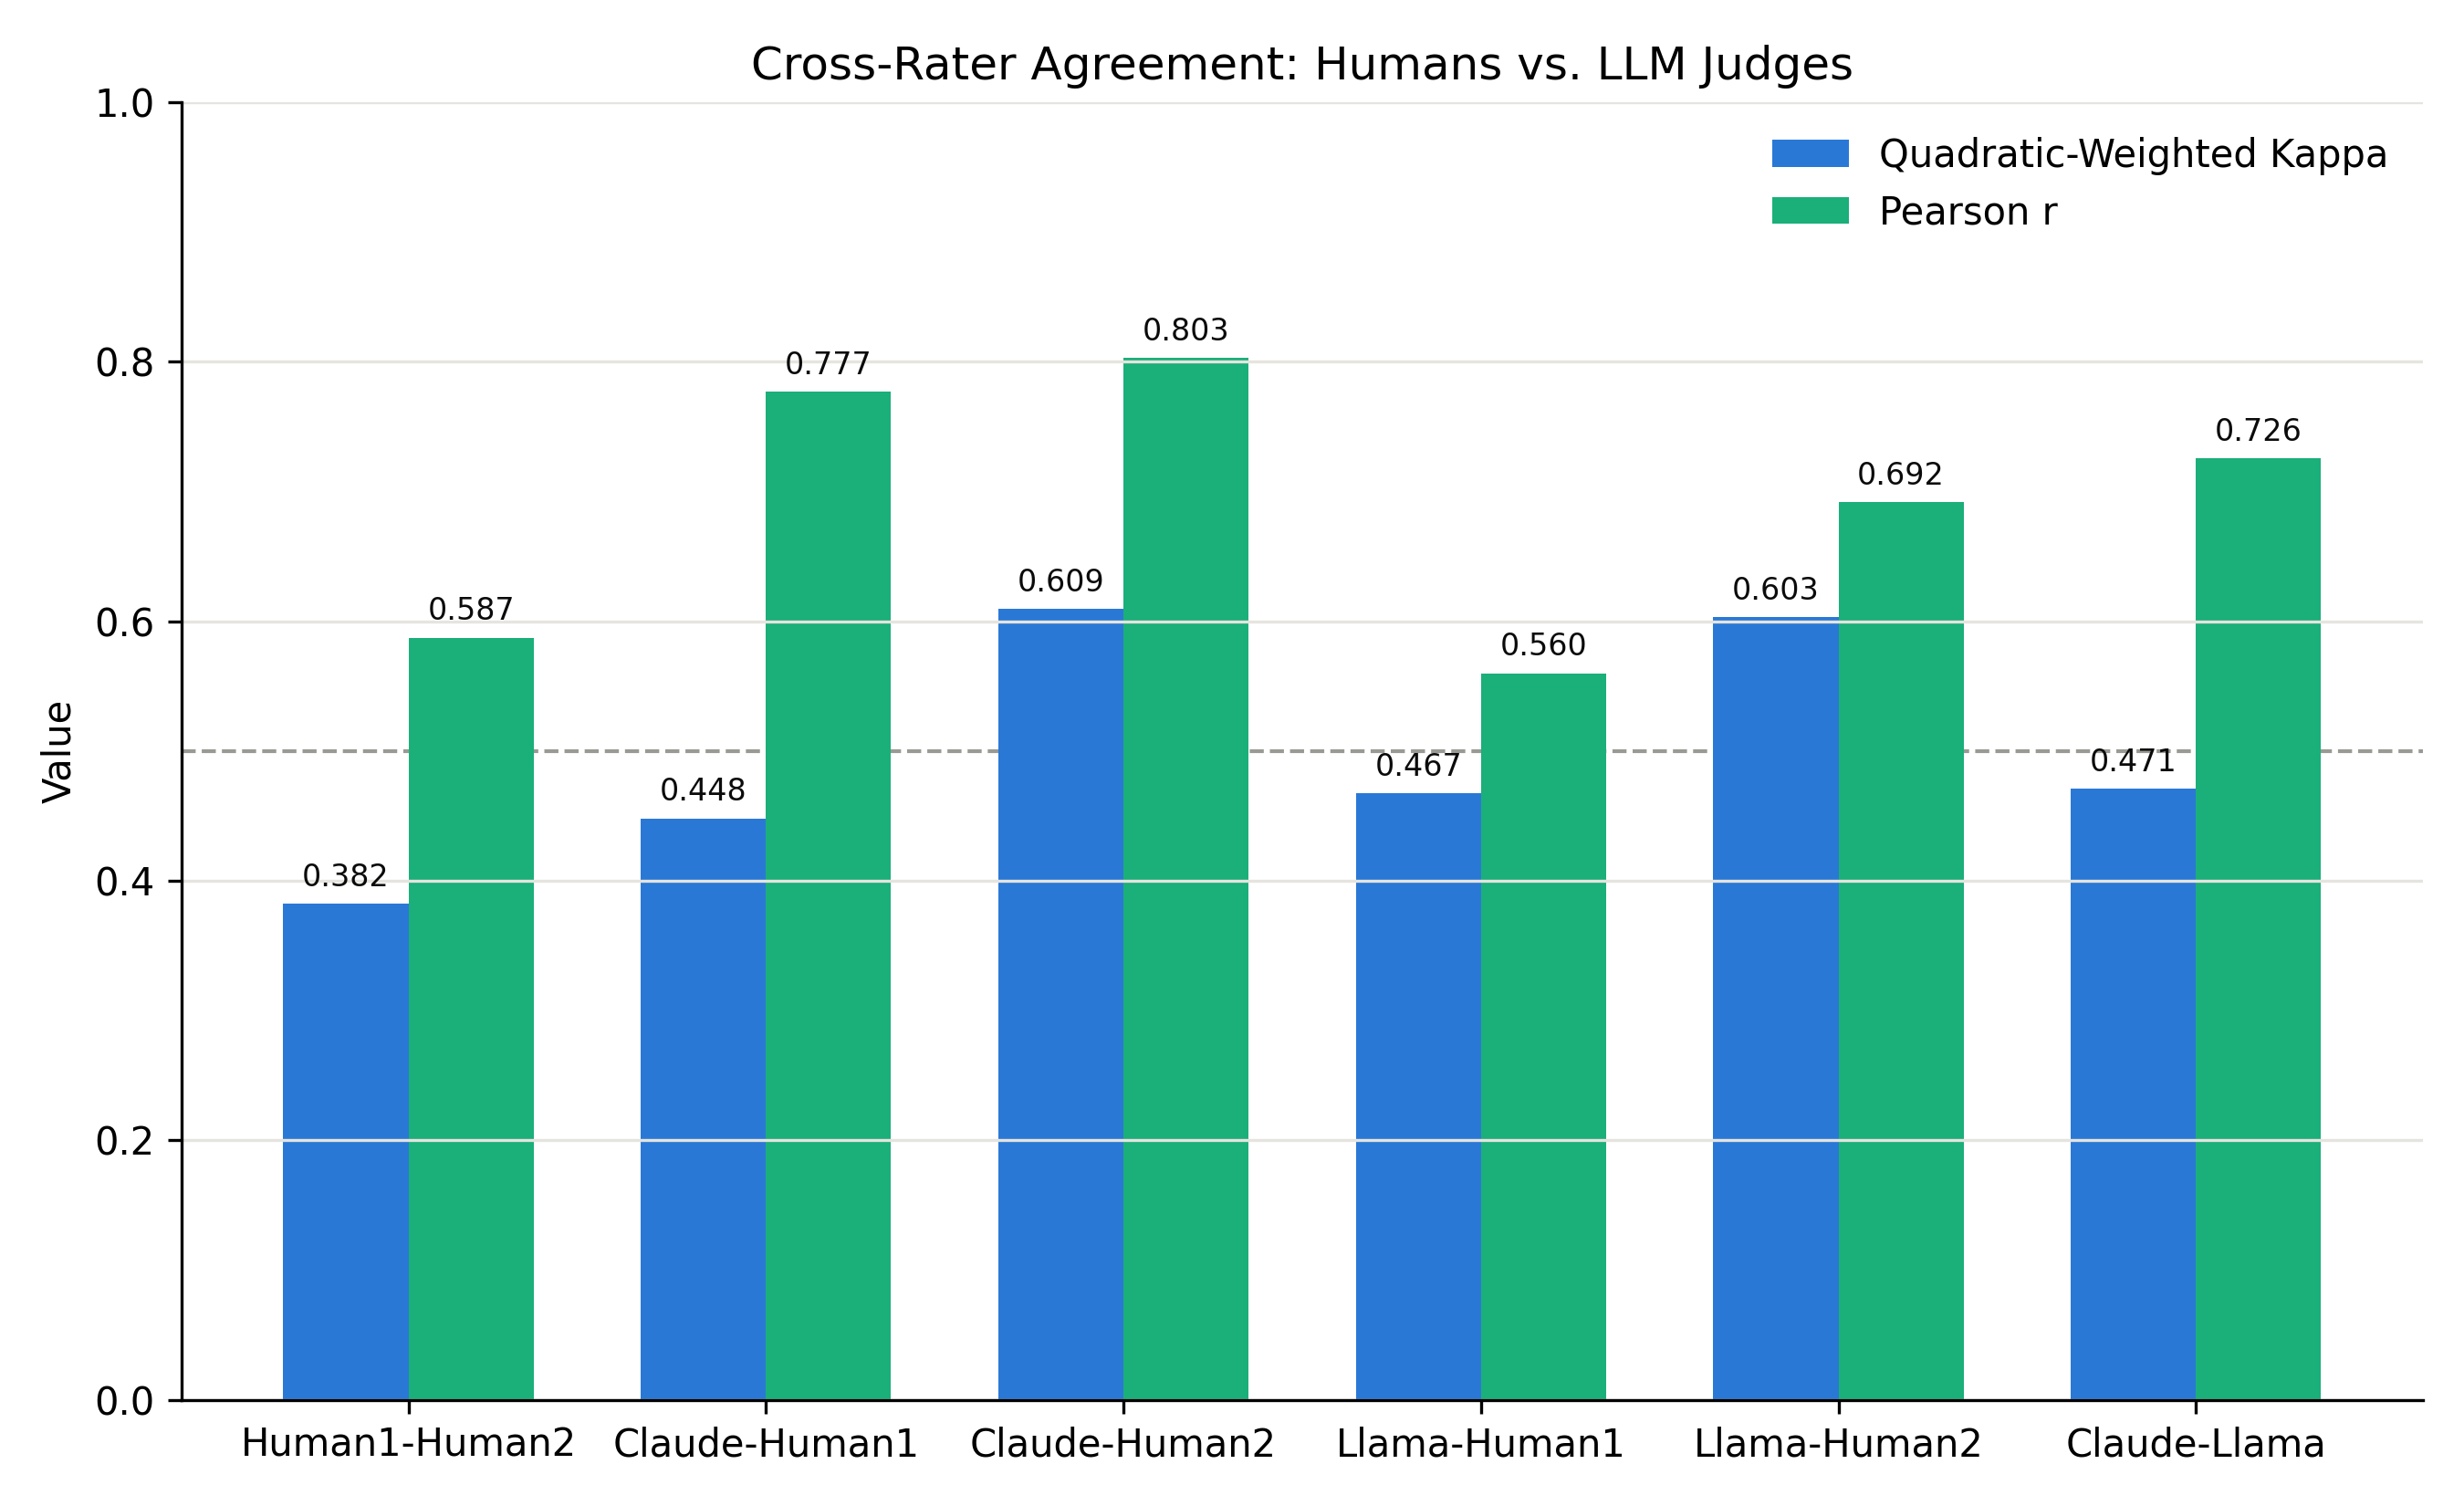
\includegraphics[width=\columnwidth]{figures/fig1_cross_rater_agreement.png}
\caption{Cross-rater agreement (quadratic-weighted Cohen's $\kappa$ and Pearson $r$) across all six rater pairs: two human annotators, the original Claude judge, and a second LLM (Llama-3.3-70B). All comparisons, including the Human1--Human2 baseline, fall within a similar range, indicating the categorical noise observed throughout the validation is inherent to the evasion construct itself rather than specific to any single rater.}
\label{fig:crossrater}
\end{figure}

\textbf{Qualitative Illustration.} Because the evasion score is a rescaled mean of four discrete 1--5 ratings, it can take 17 possible values in principle; the full corpus realizes 16 of these 17 values (only the second-highest value, 93.75, never occurs), with realizations clustered in the mid-range. Extreme scores are rare: just 3 of 3,350 pairs (0.09 percent) received the maximum score of 100, and 45 (1.34 percent) received the minimum of 0. In a representative low-evasion exchange (score = 0), management answered a detailed analyst question with specific dollar figures, per-share impacts, and a quarter-over-quarter guidance bridge; the judge's rationale credited the response with directly and comprehensively addressing all parts of the question. We define a pair as high-evasion at a threshold of evasion score $\geq 60$, consistent with the \texttt{pct\_high\_evasion} threshold used in the scoring pipeline; 95 of 3,350 pairs (2.84 percent) meet this threshold at the pair level. Such exchanges typically involve a redirect to another speaker or topic without a substantive answer to the specific question posed, consistent with the non-responsiveness dimension of the rubric.

\textbf{External Benchmark Validation.} The validation above is internal: it establishes that our judge agrees with our annotators. To test whether the measure carries beyond data we assembled ourselves, we applied the unmodified judge---identical prompt, model, and temperature, with no tuning to either corpus---to two independent evaluation sets. EvasionBench \cite{ma2026evasionbench} supplies earnings-call Q\&A in the same domain as our corpus; we score a random 1{,}000-pair sample (999 returned valid output). Its public release carries labels generated by the authors' fine-tuned Eva-4B-V2 model rather than human annotation, so agreement with it is \emph{cross-system agreement with a specialist model}, not external human validation, and we report it as such throughout. The CLARITY/QEvasion corpus \cite{thomas2024never} supplies the complementary case: 308 held-out U.S. political-interview exchanges, labelled by three human annotators, in a domain entirely outside corporate disclosure.

On both corpora the judge's mean score increases monotonically across the ordinal label, without ever having seen those labels (Table~\ref{tab:external}). Rank agreement is highly significant in both cases (Spearman $\rho = +0.615$, $p < 10^{-100}$ on EvasionBench; $\rho = +0.398$, $p < 10^{-12}$ on CLARITY), as is one-vs-rest discrimination of the most-evasive class (AUROC $0.856$, 95\% CI $[0.771, 0.926]$ and $0.741$, $[0.639, 0.835]$; bootstrap, 2{,}000 resamples). We lead with these threshold-free statistics because they do not depend on any choice of cut point.

Converting a continuous score into discrete classes exposes a sharper and more useful result. Applying cut points fixed \emph{a priori} at the tertiles of our own corpus ($18.75$ and $31.25$), with no reference to any external label, yields Macro-F1 of $0.321$ on EvasionBench but only $0.163$ on CLARITY. Refitting the two cut points on a 30\% split and evaluating on the held-out remainder yields $0.573$ (quadratic-weighted $\kappa = 0.538$) and $0.472$ ($\kappa = 0.320$) respectively. The gap between corpora is explained by scale rather than by ordering: our corpus has a mean score of $27.50$ and EvasionBench, drawn from the same domain, $26.64$, whereas the political interviews average $45.64$. Politicians are simply more evasive than executives, so thresholds calibrated on earnings calls push nearly every interview into the top category. We therefore report the framework as an \emph{ordinal} instrument that transfers across domains while its absolute calibration does not: practitioners applying it to a new setting should expect to re-derive cut points, but can rely on the ranking.

Two further observations bear on interpretation. First, agreement is higher against EvasionBench's model-generated labels ($\rho = 0.615$) than against CLARITY's human ones ($\rho = 0.398$); part of this is domain, but part is that a fine-tuned model labels more consistently than three annotators who disagree with each other. Those annotators agree at a mean pairwise Cohen's $\kappa$ of $0.477$, with all three assigning the same fine-grained label on only 40.6\% of items---independent evidence, from a published benchmark, that the modest categorical agreement reported above is characteristic of this construct rather than a defect of our annotation. Second, EvasionBench's own fine-tuned Eva-4B attains 84.9\% Macro-F1 on their gold set. We do not present our numbers as competitive with a supervised specialist; the contribution is a continuous, interpretable, training-free measure that requires no labelled data in the target domain, and it should be read against that standard.

\begin{table}[t]
\centering
\caption{External Benchmark Evaluation. The judge is unmodified and label-blind; class means increase monotonically on both corpora.}
\label{tab:external}
\begin{tabular}{lrr}
\toprule
 & EvasionBench & CLARITY \\
\midrule
Domain & Earnings calls & Political interviews \\
Label source & Eva-4B-V2 model & Human ($n$=3) \\
Pairs scored & 999 & 308 \\
\midrule
Mean score, least evasive & 18.21 & 34.57 \\
Mean score, middle & 35.41 & 48.42 \\
Mean score, most evasive & 49.46 & 58.70 \\
\midrule
Spearman $\rho$ & $+0.615$ & $+0.398$ \\
AUROC, most-evasive & 0.856 & 0.741 \\
Macro-F1, zero-shot cuts & 0.321 & 0.163 \\
Macro-F1, fitted (held out) & 0.573 & 0.472 \\
\bottomrule
\end{tabular}
\end{table}

\textbf{Contamination and Anonymization.} Because \texttt{claude-sonnet-4-6} may have encountered these calls during pretraining, its scores could in principle reflect recall of the speaking firm rather than analysis of the exchange. We tested this directly. Across the 75 validated pairs we masked every company name, ticker, executive and analyst name, product, and place---702 spans in total, 9.4 per pair, spanning 40 companies---using named-entity recognition supplemented by an explicit pass over the ticker and speaker names recorded for each pair, and re-scored the masked text with the identical judge. Scores are stable: masked and original correlate at $r = 0.861$ (quadratic-weighted $\kappa = 0.730$), 41 of 75 scores are unchanged, and the corpus mean moves by $+1.83$ points on the 0--100 scale. Agreement with the human mean falls from $r = 0.886$ to $0.773$, which we report rather than suppress; it nonetheless remains well above the $r = 0.587$ the two annotators achieve with one another, and against the first annotator the masked judge lands at $0.582$, essentially the inter-human level. One caveat limits how much of the residual decline can be attributed to contamination: masking also removes genuine concrete detail, and vagueness is one of the four scored dimensions, so the manipulation mechanically pushes text toward the evasive end---consistent with the observed upward shift. The test cannot fully separate lost recall from lost signal, and because the confound biases it toward finding an effect, the stability we observe is a conservative result.

\textbf{Dimensional Structure.} Whether the four dimensions capture distinct constructs or one underlying trait bears directly on whether averaging them is defensible. Horn's parallel analysis on the full $3{,}350 \times 4$ matrix (1{,}000 draws) retains a single factor: the first eigenvalue of $2.628$ exceeds its 95th-percentile random benchmark of $1.062$, while the second ($0.801$) falls below its own ($1.025$). The one-factor solution accounts for 56.7\% of variance. We had anticipated a two-factor structure separating directness from hedging, and note that it is not testable with four indicators regardless of the data: a two-factor exploratory model on four variables has $-1$ degrees of freedom and is under-identified, so any solution it returns is one of infinitely many. What the correlations do show descriptively (Table~\ref{tab:dimcorr}) is that hedging is the least redundant dimension, correlating $0.244$ with deflection where the remaining pairs range from $0.521$ to $0.725$. We therefore treat near-unidimensionality as support for reporting a single composite score, and leave a properly identified test of finer structure---which would require additional dimensions---to future work.

\begin{table}[t]
\centering
\caption{Pairwise Correlations Among the Four Rubric Dimensions (Full 3,350-Pair Corpus)}
\label{tab:dimcorr}
\begin{tabular}{lrrrr}
\toprule
& NR & Vague. & Defl. & Hedg. \\
\midrule
Non-responsiveness & 1.000 & 0.725 & 0.712 & 0.446 \\
Vagueness           & 0.725 & 1.000 & 0.521 & 0.547 \\
Deflection           & 0.712 & 0.521 & 1.000 & 0.244 \\
Hedging              & 0.446 & 0.547 & 0.244 & 1.000 \\
\bottomrule
\end{tabular}
\end{table}

\textbf{Illustrative Application: Evasion and Market Reaction.} As a test case for how the framework performs when applied to a concrete downstream hypothesis, we examined whether evasion predicts subsequent market reactions. We find no significant relationship: Pearson correlations between evasion measures and three-day CAR are small and non-significant (mean evasion: $r = -0.030$, $p = 0.714$; variance: $r = +0.047$, $p = 0.560$; max: $r = +0.008$, $p = 0.920$), a pattern that holds under the rank-based Spearman correlation as well (mean evasion: $\rho = -0.008$, $p = 0.920$; variance: $\rho = +0.019$, $p = 0.817$; max: $\rho = +0.013$, $p = 0.871$), as shown in Figure~\ref{fig:evasioncar}, and adding evasion measures to a classification model predicting earnings-surprise direction (Table~\ref{tab:auroc}) offers no reliable improvement once uncertainty is accounted for. The point estimate for the Config C minus Config B AUROC difference is $+0.034$ for logistic regression (bootstrap 95\% CI: $[-0.017, +0.086]$) and $+0.006$ for XGBoost (95\% CI: $[-0.072, +0.083]$); both intervals include zero. This is further confirmed by 5-fold cross-validation (Config B vs.\ C mean AUROC: 0.508 vs.\ 0.508 logistic regression, 0.528 vs.\ 0.529 XGBoost; both $p > 0.90$). We report this null result as an honest boundary condition: within this sample, size, and application, the framework's evasion scores do not carry incremental financial predictive content, a finding we examine further in Section~\ref{sec:robustness}.

\begin{figure}[t]
\centering
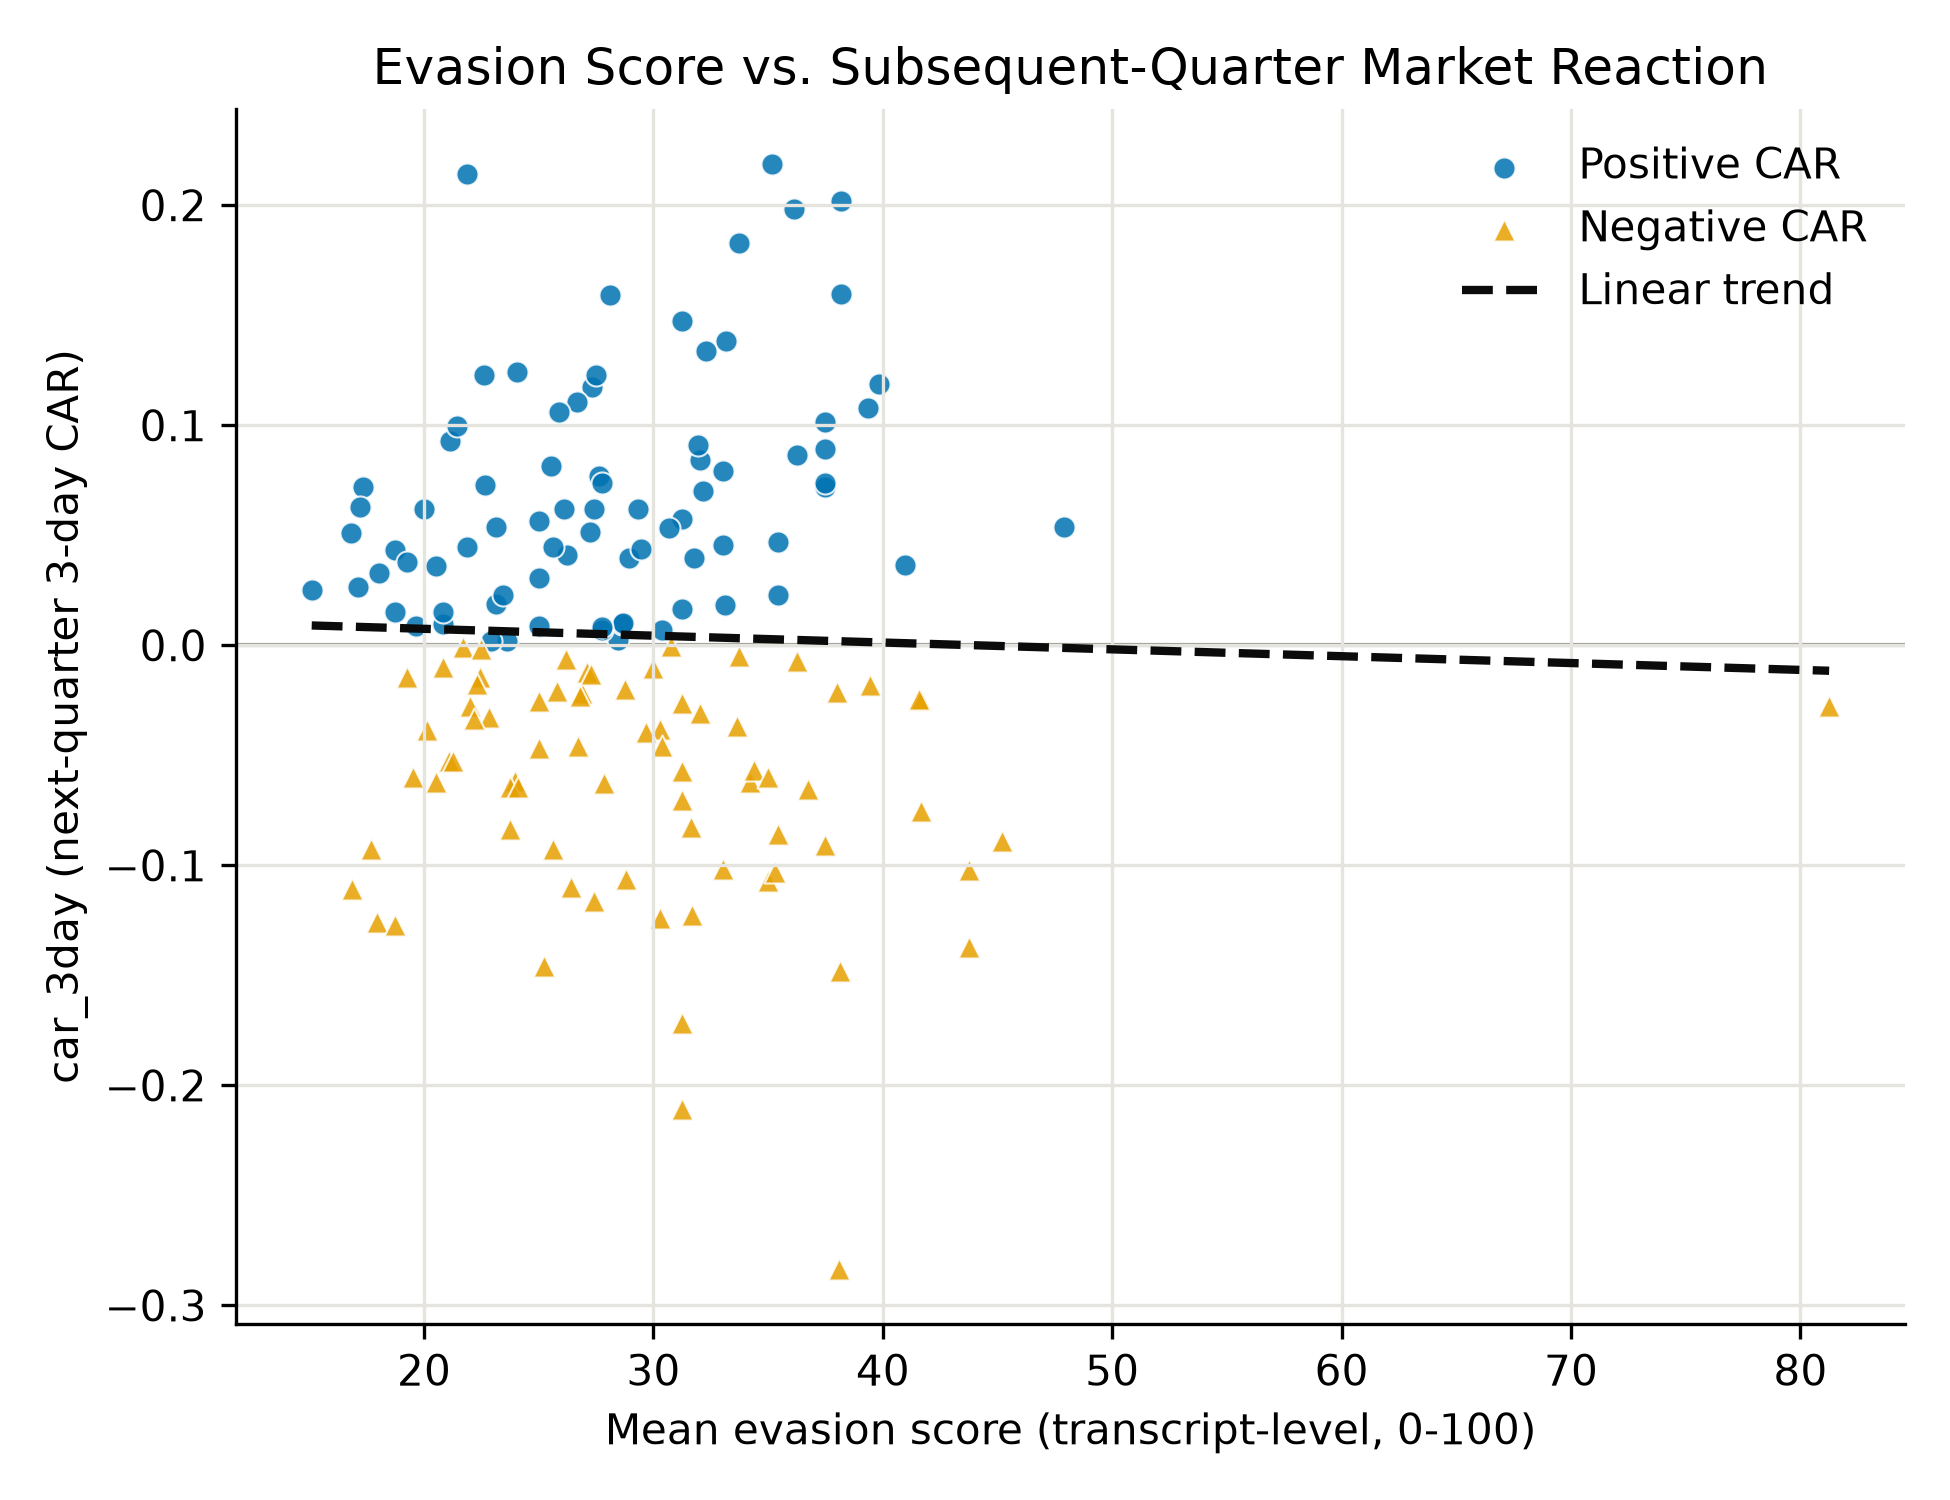
\includegraphics[width=\columnwidth]{figures/fig2_evasion_vs_car.png}
\caption{Mean transcript-level evasion score versus subsequent-quarter three-day CAR ($n$=155). The dashed trend line reflects the near-zero correlation reported in the text ($r = -0.030$).}
\label{fig:evasioncar}
\end{figure}

\begin{table}[t]
\centering
\caption{Illustrative Application: Out-of-Sample AUROC by Configuration}
\label{tab:auroc}
\begin{tabular}{lrr}
\toprule
Configuration & LR AUROC & XGB AUROC \\
\midrule
A: Accounting only & 0.486 & 0.512 \\
B: A + LM sentiment & 0.608 & 0.414 \\
C: B + mean evasion & 0.642 & 0.420 \\
D: B + all evasion measures & 0.629 & 0.384 \\
\bottomrule
\end{tabular}
\\[4pt]
\footnotesize C$-$B difference, bootstrap 95\% CI: LR $+0.034$ $[-0.017, +0.086]$; XGB $+0.006$ $[-0.072, +0.083]$
\end{table}

\section{Robustness and Additional Analysis}
\label{sec:robustness}

We ran 5-fold stratified cross-validation on Configs B and C (Table~\ref{tab:cv}) to characterize the null result rigorously rather than reporting a single specification. Mean AUROC is statistically indistinguishable across configurations for both model types, and fold-to-fold SD (0.075--0.165) dwarfs the single-split point estimate, confirming the result reflects sampling variance rather than a stable effect.

Because the 2015--2023 sample spans a period of extreme, largely firm-independent volatility, we re-estimated all specifications excluding 2020 (25 observations); results are essentially unchanged ($r = 0.002$, $p = 0.982$, $n = 130$; AUROC shifts of 0.01 or less), so the null result is not a COVID-era artifact. A post-hoc power analysis indicates that at $n = 155$, this design has 7.0, 12.9, 34.4, and 66.4 percent power to detect true AUROC differences of 0.02, 0.05, 0.10, and 0.15 respectively, none reaching conventional thresholds: the data rule out a moderate-to-large effect but remain underpowered for smaller ones, a limitation of sample size rather than of the framework itself. A SHapley Additive exPlanations analysis of the best XGBoost specification ranks return on assets as most influential, followed by revenue growth and the two margin measures, with evasion measures absent from that configuration entirely, consistent with the cross-validated null result.

\begin{table}[t]
\centering
\caption{5-Fold Cross-Validation AUROC, Configs B and C}
\label{tab:cv}
\begin{tabular}{lrrrr}
\toprule
& \multicolumn{2}{c}{Logistic Regression} & \multicolumn{2}{c}{XGBoost} \\
Fold & Config B & Config C & Config B & Config C \\
\midrule
1 & 0.483 & 0.425 & 0.579 & 0.533 \\
2 & 0.313 & 0.358 & 0.413 & 0.433 \\
3 & 0.708 & 0.621 & 0.558 & 0.558 \\
4 & 0.642 & 0.679 & 0.471 & 0.488 \\
5 & 0.396 & 0.458 & 0.617 & 0.633 \\
\midrule
Mean & 0.508 & 0.508 & 0.528 & 0.529 \\
SD & 0.165 & 0.136 & 0.084 & 0.075 \\
\bottomrule
\end{tabular}
\end{table}

Because the 155-observation panel spans only 32 firms with repeated observations per firm, standard errors that ignore this clustering may understate uncertainty. We re-estimated the Config C logistic specification with standard errors clustered by firm: the coefficient on mean evasion score remains non-significant under both naive ($p = 0.083$) and firm-clustered ($p = 0.054$) standard errors, confirming the null result is not an artifact of ignoring within-firm correlation.

The pairwise correlations among the four rubric dimensions are reported in Section~\ref{sec:results}. One caveat belongs here: ``deflection'' appears as a labeled dimension in both our LLM rubric and the parallel human validation rubric, which may modestly inflate convergence on that dimension relative to a fully independent instrument.

Finally, to assess whether the evasion score reflects a stable construct rather than an artifact of specific prompt wording, we re-scored the 75-pair validation sample using two additional prompt variants: one rewording the rubric's dimension descriptions, and one reordering the four dimensions within the prompt. Both variants correlate strongly with the original scores (reworded: $r = 0.928$, $p < 0.001$, quadratic-weighted $\kappa = 0.847$; reordered: $r = 0.890$, $p < 0.001$, quadratic-weighted $\kappa = 0.682$), indicating the evasion construct is stable under reasonable prompt variation rather than reflecting a single phrasing's idiosyncrasies.

We report a large number of correlations and AUROC contrasts across Sections~\ref{sec:results}--\ref{sec:robustness}. We do not apply a formal multiple-comparisons correction, both because nearly every reported contrast fails to cross conventional significance thresholds even uncorrected, which a correction would only reinforce, and because our stance throughout is to report every specification we ran rather than a favorable subset; a correction would matter more if we were selecting among many tests for a positive result, which we explicitly are not doing here.

Because the judge model was trained on public web text that plausibly includes some of these 2015--2023 SEC transcripts, a natural concern is training-data contamination: could the model's parametric memory of a company's subsequent performance, rather than the text presented to it, be tinting its evasion score? We consider this a lower-risk form of contamination than factual recall tasks, since the judge is asked to rate specific textual features of the presented question-response pair (directness, hedging language, deflection) rather than to recall or predict an outcome, and the prompt explicitly withholds market and outcome information (Section~\ref{sec:results}). We nonetheless flag this as a residual concern rather than a resolved one; a company-anonymized or lightly paraphrased robustness check, showing scores are stable when identifying details are removed, would directly address it and is a natural addition for a future revision.

\textbf{Limitations.} We summarize the main limitations of this study explicitly. The primary judge is a single LLM (\texttt{claude-sonnet-4-6}); Section~\ref{sec:results}'s cross-model comparison and the prompt-robustness check above both suggest the construct generalizes across models and prompt wordings, though both checks were conducted on the same 75-pair subsample rather than the full corpus. Human validation relies on two annotators who are also this paper's student authors, working blind to model output but drawn from a small, non-independent pool; a larger and more diverse annotator panel would strengthen this further. The financial application's panel is modest (155 observations, 32 firms) and firm concentration, while improved from an earlier iteration of this dataset, remains a relevant caveat despite firm-clustered standard errors confirming the null result's robustness to this concern. The evasion score itself is compressed (16 of 17 possible pair-level values realized, with the transcript-level means used in the financial application clustered between roughly 20 and 35), which limits the amount of downstream variation available to any predictive model. The CAR measure used is market-adjusted rather than risk-adjusted, some earnings announcement dates are estimated rather than directly observed (flagged via \texttt{car\_date\_estimated}), and the realized company panel, drawn from EDGAR full-text search rather than a pre-specified sector universe, skews toward industrials and services rather than the technology and healthcare sectors originally targeted; readers should weigh generalizability accordingly.

\textbf{Positioning relative to comparable published work.} The closest published antecedents to our financial application, Larcker and Zakolyukina~\cite{larcker2012detecting} and Gow et al.~\cite{gow2021nonanswers}, both appearing in the \emph{Journal of Accounting Research}, and Barcellos~\cite{barcellos2025overcoming}, in \emph{Management Science} (DOI: 10.1287/mnsc.2025.01197), draw on far larger conference-call samples (hundreds to thousands of firm-quarters) than our 155-observation illustrative panel. We do not claim parity with those samples; rather, we position this paper's contribution as the validated measurement framework itself, with the financial application serving as a rigorously-reported test case rather than a claim of comparable statistical power. Extending the framework to a sample of that scale is the natural next step and the most direct path to a stronger financial contribution.

\section{Conclusion}

This paper introduces and validates a structured LLM-as-judge framework for measuring evasion in adversarial institutional question-and-answer exchanges, applied at scale to 3,350 real question-response pairs from 285 SEC-filed earnings call transcripts and validated against independent human annotation. The framework's evasion scores correlate meaningfully with human judgment on a continuous scale, even where categorical agreement is more modest, extending the LLM-as-judge paradigm from its established use in benchmarking generative model outputs to detecting strategic communicative behavior in real institutional settings. As an illustrative test of a concrete downstream application, we examined whether evasiveness predicts subsequent market reactions to earnings announcements and found no significant relationship, a result stable under cross-validation and robust to excluding the COVID-19 period; a formal power analysis indicates this reflects the limits of this specific sample rather than definitive evidence against any relationship at any scale. We regard this as a successful demonstration of how the framework should be applied and evaluated rigorously, not as a verdict on its value.

We see the framework's more general contribution as extending well beyond corporate earnings calls: any adversarial institutional Q\&A setting---legislative testimony, regulatory hearings, press conferences by public officials---presents a natural application for a validated, scalable, human-interpretable measure of evasiveness. Future work applying this framework to a substantially larger and more diverse financial sample would help determine whether the null result reported here reflects a genuine absence of relationship or the statistical limits of the present study.

\section*{Data and Code Availability}

All code, data pipeline scripts, and results underlying this paper are publicly available at \url{https://github.com/kunalchevuri/question-evasion-detection-LLM-framework_research} (commit \texttt{d23b919}). All data sources used (SEC EDGAR filings, Yahoo Finance price data, SEC XBRL structured data, the Loughran-McDonald dictionary) are free and publicly accessible. The repository README provides step-by-step reproduction instructions, with \texttt{final\_verification.py} as the primary entry point for reproducing all headline statistics reported in this paper.

\section*{Acknowledgments}

We thank the U.S. Securities and Exchange Commission for maintaining the freely accessible EDGAR system and the developers of the Loughran--McDonald sentiment dictionary, without which this paper's data pipeline would not have been possible.

\section*{Responsible Use}

The evasion score introduced here is a research instrument, not a verdict: a high score reflects the presence of textual features associated with non-responsiveness, vagueness, deflection, or hedging, and can arise from legitimate reasons (active litigation, trade-secret protection, or genuine uncertainty) as well as strategic evasion. We caution against using this or any similar automated score as a standalone basis for market-moving claims about a specific company or executive, including in short-selling or activist campaigns; it is intended as one input among many for researchers studying disclosure behavior in aggregate, not as an individual-transcript verdict.

\section*{Generative AI Use and Conflict of Interest Statement}

Large language models (Claude, Llama 3.3 70B) are core methodological instruments in this study, not writing aids; their role, prompting, and evaluation are described in full in Sections~\ref{sec:methodology}--\ref{sec:robustness}. Generative AI coding assistants were used during development of the data pipeline and analysis scripts underlying this paper; all resulting code, intermediate outputs, and headline statistics were independently verified by the authors against the committed data before inclusion, as detailed in the Data and Code Availability statement. M. Aledhari is both a co-author and the student authors' research advisor; the authors declare no other financial or non-financial conflicts of interest related to this work.

\bibliographystyle{IEEEtran}
\bibliography{refs}

\end{document}
